\chapter{KHẢO SÁT HỆ THỐNG ĐO NHIỆT ĐỘ}

\section{Mục đích}
\begin{itemize}
	\item Tìm hiểu các thành phần của hệ thống đo nhiệt độ.
	\item Nắm vững một số nội dung tính toán liên quan đến thiết kế hệ thống đo nhiệt độ.
\end{itemize}

\section{Dụng cụ}
\begin{itemize}
	\item Hệ thống đo và điều khiển nhiệt độ.
	\item Nhiệt kế chất lỏng; vòng gia nhiệt; oscilloscope.
	\item Khối kim loại làm đều nhiệt và đặt cặp nhiệt điện, nhiệt kế chất lỏng.
\end{itemize}

\section{Các bước tiến hành thí nghiệm}
\begin{table}[ht]
	\centering
	\caption{Bảng đo độ dài theo chiều tăng giảm lực bằng đồng hồ so 0.01mm}
	\begin{tabular}{lp{4cm}ll}\toprule
		STT & Nhiệt độ nhiệt kế chất lỏng ($ ^\circ $) & Chiều giảm lực & Chiều tăng lực\\\midrule
		1 & 90 & 2.73 & 2.57 \\
		2 & 120 & 3.88 & 3.69 \\
		3 & 150 & 5.08 & 4.89 \\
		4 & 180 & 6.29 & 6.04 \\
		5 & 210 & 7.35 & 7.63 \\
		6 & 240 & 8.46 & 8.50 \\
		7 & 270 & 9.65 & 9.61 \\
		8 & 300 & 10.85 & 10.83 \\\bottomrule
	\end{tabular}
\end{table}

\section{Báo cáo}
\begin{figure}[ht]
	\centering
	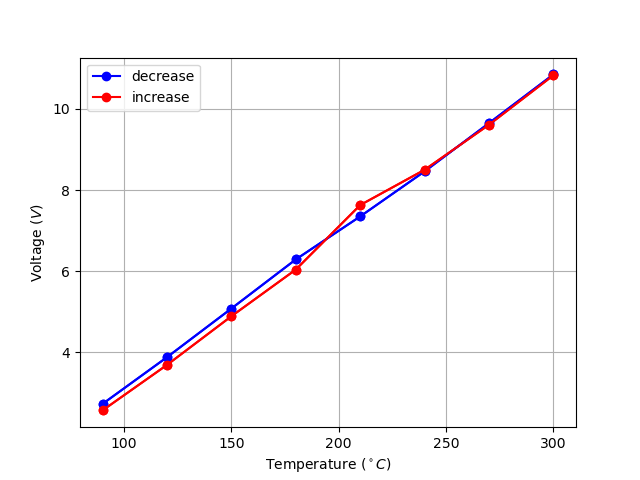
\includegraphics[width=0.8\linewidth]{Figure_1.png}
	\caption{Đường đặc tuyến cặp nhiệt khi tăng và giảm nhiệt độ}
\end{figure}

Nhận xét:
\begin{itemize}
	\item Hai đường đặc tuyến gần như là đường thẳng.
	\item Đường đặc tuyến khi giảm nhiệt nằm trên đường đặc tuyến khi tăng nhiệt.
\end{itemize}